\chapter{CI / CD}
\section{Was ist CI/CD}

Es handelt sich hier um Methode, bei der den Kunden regelmäßig Apps bereitgestellt und alle Phasen der Anwendungsentwicklung automatisiert werden. Die Hauptkonzepte von CI/CD sind Continuous Integration, Continuous Delivery und Continuous Deployment. CI/CD löst die Probleme, welche die Integration von neuem Code für DevOps-Teams verursachen kann.\cite{whatIsCICD}

Insbesondere sorgt CI/CD für eine kontinuierliche Automatisierung und Überwachung über den gesamten App-Lifecycle hinweg, von der Integrations- und Test- bis hin zur Bereitstellungs- und Implementierungsphase. Diese zusammenhängenden Praktiken werden oft als „CI/CD-Pipeline“ bezeichnet, und sie werden durch eine agile Zusammenarbeit der DevOps-Teams unterstützt.\autocite{whatIsCICD}

Die Abkürzung CI/CD hat unterschiedliche Bedeutungen. „CI“ bedeutet Continuous Integration, also der Automatisierungsprozess für Entwickler. Bei einer erfolgreichen CI werden regelmäßig neue Codeänderungen für Apps entwickelt, geprüft und in einem gemeinsamen Repository zusammengeführt. Damit soll der Konflikt verhindert werden, den zu viele Branches einer App verursachen können, wenn sie zeitgleich entwickelt werden.\autocite{whatIsCICD}

„CD“ bedeutet Continuous Delivery bzw. Continuous Deployment. Dass sind verwandte Konzepte, die zuweilen synonym verwendet werden. Obwohl es bei beiden Konzepten um die Automatisierung weiterer Phasen der Pipeline geht, werden die Begriffe manchmal unterschiedlich verwendet, um das Ausmaß der Automatisierung zu verdeutlichen.\autocite{whatIsCICD}

Continuous Delivery bedeutet üblicherweise, dass App-Änderungen eines Entwicklers automatisch auf Bugs getestet und in ein Repository (wie GitHub oder eine Container-Registry) hochgeladen werden, von wo aus sie vom Operations-Team in einer Live-Produktivumgebung bereitgestellt werden können. Dieser Vorgang ist die Antwort auf Transparenz- und Kommunikationsprobleme zwischen Dev- und Business-Teams. Damit soll sichergestellt werden, dass neuer Code mit minimalem Aufwand implementiert werden kann.\autocite{whatIsCICD}

Continuous Deployment (das andere „CD“) kann sich auf die automatische Freigabe von Entwickleränderungen vom Repository zur Produktivphase beziehen, wo sie direkt vom Kunden genutzt werden können. Dieser Vorgang soll der Überlastung von Operations-Teams bei manuellen Prozessen entgegenwirken, die die Anwendungsbereitstellung verlangsamen. Continuous Development baut die Vorteile der Continuous Delivery aus, indem auch noch die nächste Phase der Pipeline automatisiert wird.\autocite{whatIsCICD}

\begin{figure}[h]
	\centerline{
		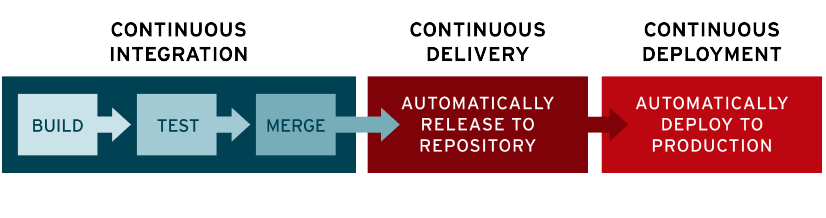
\includegraphics[width=0.8\textwidth]{./grafiken/ci-cd-flow-redhatsource.png}
	}
	\vskip0pt
	\caption{CI/CD Workflow (Bild wurde entnommen aus \cite{whatIsCICD})}
\end{figure}


Manchmal sind mit CI/CD lediglich die zusammenhängenden Praktiken der Continuous Integration und der Continuous Delivery, manchmal aber auch alle drei Konzepte der Continuous Integration, Continuous Delivery und Continuous Deployment gemeint. Noch komplizierter wird das Ganze dadurch, dass mit Continuous Delivery zuweilen auch die Prozesse des Continuous Deployment mitgemeint sind.\autocite{whatIsCICD}

Letztendlich bringen uns diese Details jedoch nicht weiter. Sehen Sie CI/CD einfach als Prozess an, der nicht selten als Pipeline visualisiert wird und der ein hohes Maß an kontinuierlicher Automatisierung und Überwachung bei der Anwendungsentwicklung umfasst. Je nach Fall hängt die Auslegung des Begriffs vom Grad der Automatisierung der CI/CD-Pipeline ab. Viele Unternehmen arbeiten zunächst mit CI und setzen den Prozess später mit der automatischen Bereitstellung und Implementierung fort, z. B. bei cloudnativen Apps.\autocite{whatIsCICD}

\section{Continuous Integration}

Bei der modernen Anwendungsentwicklung arbeiten mehrere Entwickler an unterschiedlichen Features der gleichen App. Die gleichzeitige Zusammenführung aller Quellcode-Branches an einem Tag (auch bekannt als „Merge Day“) kann einen hohen Arbeits- und Zeitaufwand bedeuten. Der Grund dafür ist, dass Anwendungsänderungen von getrennt arbeitenden Entwicklern miteinander in Konflikt treten können, wenn sie zeitgleich durchgeführt werden. Dieses Problem kann sich verschlimmern, wenn jeder Entwickler seine eigene lokale Integrated Development Environment (IDE) definiert, statt im Team eine gemeinsame cloudbasierte IDE zu erstellen.\autocite{whatIsCICD}

Mithilfe der Continuous Integration (CI) können Entwickler ihre Codeänderungen in einem gemeinsamen „Branch“ oder „Trunk“ der Anwendung viel häufiger zusammenführen, manchmal sogar täglich. Sobald die Änderungen eines Entwicklers zusammengeführt werden, werden sie in automatischen App-Builds und unterschiedlichen Stufen von Automatisierungsprüfungen (normalerweise Einheits- und Integrationstests) validiert. So wird sichergestellt, dass die Funktionsfähigkeit nicht beeinträchtigt wurde. Dabei müssen alle Klassen und Funktionen bis hin zu den verschiedenen Modulen der App getestet werden. Wenn die automatische Prüfung Konflikte zwischen aktuellem und neuem Code erkennt, lassen sich diese mithilfe von CI schneller und häufiger beheben.\autocite{whatIsCICD}

\section{Continuous Delivery}

Nach der Automatisierung von Builds und Einheits- und Integrationstests bei der CI wird bei der Continuous Delivery auch die Freigabe des validierten Codes an ein Repository automatisch durchgeführt. Um also einen effizienten Continuous Delivery-Prozess zu gewährleisten, muss die CI bereits in Ihre Entwicklungs-Pipeline integriert sein. Ziel der Continuous Delivery ist eine Codebasis, die jederzeit in einer Produktivumgebung bereitgestellt werden kann.\autocite{whatIsCICD}

Bei der Continuous Delivery umfasst jede Phase − von der Zusammenführung der Codeänderungen bis zur Bereitstellung produktionsreifer Builds − automatisierte Tests und Code-Freigaben. Am Ende dieses Prozesses kann das Operations-Team eine App schnell und einfach in der Produktivphase bereitstellen.\autocite{whatIsCICD}

\section{Continuous Deployment}

Die abschließende Phase der CI/CD-Pipeline ist das Continuous Deployment. Als Erweiterung der Continuous Delivery, bei der produktionsreife Builds automatisch an ein Code-Repository freigegeben werden, wird beim Continuous Deployment auch die Freigabe einer App in die Produktivphase automatisiert. Da der Produktivphase in der Pipeline kein manuelles Gate vorgeschaltet ist, müssen beim Continuous Deployment die automatisierten Tests immer sehr gut durchdacht sein.\autocite{whatIsCICD}

In der Praxis bedeutet Continuous Deployment, dass App-Änderungen eines Entwicklers binnen weniger Minuten nach ihrer Erstellung live gehen können (vorausgesetzt, sie bestehen den automatischen Test). Dies erleichtert eine kontinuierliche Integration von User Feedback ungemein. All diese zusammenhängenden CI/CD-Praktiken machen eine Anwendungsimplementierung weniger riskant, weil Änderungen in Teilen und nicht auf einmal freigegeben werden. Die Vorabinvestitionen sind allerdings beträchtlich, da automatische Tests für die diversen Prüf- und Release-Phasen in der CI/CD-Pipeline geschrieben werden müssen.\autocite{whatIsCICD}

\section{GitLab Pipeline}

Pipelines sind top-level Komponenten der Continuous Integration, Delivery und Deployment. Pipelines umfassen:\autocite{gitlabPipelines}

\begin{itemize}
	\item Jobs, welche definieren \textit{was} auszuführen ist. Zum Beispiel gibt es Jobs, welche den Code kompilieren, Packete installieren und testen.
	\item Stages, welche definieren \textit{wann} Jobs auszuführen sind. Beispielsweise ist die Kompile-Stage üblicherweise vor der Test-Stage.
\end{itemize}

Jobs werden von Runner ausgeführt. Mehrere Jobs in der selben Stage werden parallel ausgeführt, wenn genügend simultane Runner bereitstehen.
Wenn \textit{alle} Jobs in einer Stage erfolgreich ausgeführt wurden, geht die Pipeline zur nächsten Stage über.
Wenn \textit{irgendein} Job in einer Stage fehlschlägt, wird die nächste Stage (normalerweise) nicht ausgeführt und die Pipeline endet vorzeitig.\autocite{gitlabPipelines}

\newpage

Im Allgemeinen werden Pipelines in der Regel automatisch  nach dem Hochladen eines Commits ausgeführt und erfordern nach ihrer Erstellung keinen weiteren manuellen Eingriff.
Eine typische Pipeline kann aus vier Phasen bestehen, die in der folgenden Reihenfolge ausgeführt werden:\autocite{gitlabPipelines}

\begin{itemize}
	\item Eine \colorbox{lightgray}{\texttt{Build-Stage}}, mit einem \colorbox{lightgray}{\texttt{Compile-Job}}.
	\item Eine \colorbox{lightgray}{\texttt{Test-Stage}}, welche mehrere \colorbox{lightgray}{\texttt{Test-Jobs}} beinhalten kann.
	\item Eine \colorbox{lightgray}{\texttt{Staging-Stage}}, mit einem \colorbox{lightgray}{\texttt{Deploy-to-Stage-Job}}.
	\item Eine \colorbox{lightgray}{\texttt{Production-Stage}}, mit einem \colorbox{lightgray}{\texttt{Deploy-to-Production-Job}}.
\end{itemize}

\section{GitLab Runner} \label{sec:lblGitLabRunner}
\subsection{Registrierung}

GitLab Runner ist eine Anwendung, die mit GitLab CI/CD arbeitet, um Aufträge in einer Pipeline auszuführen.
Man kann die GitLab Runner-Anwendung auf der Infrastruktur installieren, die man besitzen oder verwalten. In diesem Fall sollte man GitLab Runner auf einem Rechner installieren, der von dem Rechner getrennt ist, der die GitLab-Instanz hostet. GitLab Runner ist Open-Source und in Go geschrieben. Er kann als einzelne Binärdatei ausgeführt werden, wobei es keine sprachspezifischen Anforderungen benötigt.
Es ist auch möglich, GitLab Runner auf verschiedenen unterstützten Betriebssystemen installieren. Andere Betriebssysteme sind ebenfalls in der Lage Runner bereitzustellen, sofern diese eine Go-Binärdatei kompilieren können.
GitLab Runner kann auch in einem Docker-Container ausgeführt oder in einem Kubernetes-Cluster bereitgestellt werden.\autocite{gitlabRunner}

\begin{figure}[h]
	\centerline{
		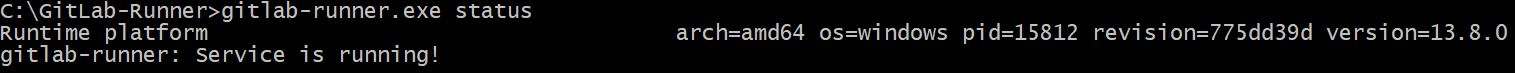
\includegraphics[width=1.1\textwidth]{./grafiken/gitlab_runner_status.JPG}
	}
	\vskip0pt
	\caption{GitLab Runner Instanz auf einem lokalen Windows-Rechner}
\end{figure}

\subsection{Executors} \label{sssec:lblExecutor}

Wenn Sie einen Runner registrieren, müssen Sie einen Executor auswählen. Ein Executor bestimmt die Umgebung, in der jeder Job läuft.\autocite{gitlabRunner}

Wenn man zum Beispiel will, dass ein CI/CD-Auftrag PowerShell-Befehle ausführt, kann man GitLab Runner auf einem Windows-Server installieren und dann einen Runner registrieren, der den Shell-Executor verwendet.
Wenn man möchte, dass ein CI/CD-Job Befehle in einem benutzerdefinierten Docker-Container ausgeführt wird, muss man GitLab Runner auf einem Linux-Server installieren und einen Runner registrieren, der den Docker-Executor verwendet.
Dies sind nur einige der möglichen Konfigurationen. Man könnte GitLab Runner auch auf einer virtuellen Maschine installieren und eine andere virtuelle Maschine als Executor verwenden lassen.
Wenn man GitLab Runner in einem Docker-Container installieren und den Docker-Executor für die Ausführung der Jobs auswählen, wird dies manchmal als "Docker-in-Docker"-Konfiguration bezeichnet.\autocite{gitlabRunner}

\subsection{Shared Runners}

Shared Runners sind für jedes Projekt in einer GitLab-Instanz verfügbar.

Shared Runners werden verwendet, wenn man mehrere Jobs mit ähnlichen Anforderungen in mehreren Projekten hat. Also anstatt viele Runner für viele Projekte im Leerlauf zu haben, kann man eine Gruppe von Runner für alle Projekte benützen.\autocite{gitlabSharedRunner}

\subsection{Tags}

Registrierte Runner kann man sogenannte Tags zuweisen. Wenn ein CI/CD Job läuft, kann dieser anhand seiner zugewiesener Tags determinieren, welchen Runner er verwenden soll. Das hat den Vorteil, dass man für beispielsweise einen Job, der ein Ruby Projekt kompilieren soll, seinen Runner nicht umkonfigurieren muss, sondern automatisch der Ruby-Runner verwendet wird.

Man muss dazu lediglich folgendes in seine  \colorbox{lightgray}{\texttt{.gitlab-ci.yml}} Datei einbinden:

\begin{figure}[h]
	\centerline{
		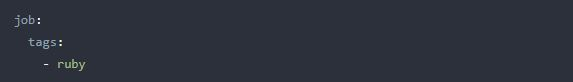
\includegraphics{./grafiken/ruby_runner_tag_in_gitlab-ci-yml_file.JPG}
	}
	\vskip0pt
	\caption{ruby Tag in gitlab-ci.yml Datei (Bild wurde entnommen aus \autocite{gitlabRunner})}
\end{figure}

\newpage

\section{MyPöttinger GitLab Pipeline}

Die Umgestaltung der GitLab Pipeline für das MyPöttinger-Repository ist ein wichtiger Bestandteil der Diplomarbeit. Die neue Pipeline besteht aus drei Stages:

\begin{itemize}
	\item Der \colorbox{lightgray}{\texttt{Build-Stage}}
	\item Der \colorbox{lightgray}{\texttt{Test-Stage}}
	\item Der \colorbox{lightgray}{\texttt{Release-Stage}}
\end{itemize}

\subsection{Die {\texttt{gitlab-ci.yml}} - Datei }

Die \texttt{gitlab-ci.yml} Datei ist in GitLab hauptverantwortlich für das CI/CD Geschehen. Sie beschreibt die Aufgaben der einzelnen Jobs, definiert in welcher Stage diese auszuführen sind und legt die Reihenfolge der Abarbeitung klar fest. Bevor man sich über die \texttt{gitlab-ci.yml} Datei Gedanken macht, ist es wichtig, auf mehrere Aspekte zu achten. Man muss sich überlegen, welchen Runner[\ref{sec:lblGitLabRunner}] man verwenden will, welchen Executor[\ref{sssec:lblExecutor}] dieser ausführt und in welcher Umgebung alles stattfindet.

Zu Beginn der gitlab-ci.yml Datei muss man definieren, in welcher Umgebung Befehle ausgeführt werden sollen. Für MyPöttinger ist standardmäßig das \texttt{mcr.microsoft.com/dotnet/sdk:5.0} Image von Microsoft gewählt, da diese bereits .NET CLI, .NET runtime und ASP.NET Core bereit stellt, welche alle für das Kompilieren, Bauen und Veröffentlichen einer .NET-Applikation benötigt werden.

\begin{lstlisting}[caption={Erste Zeilen der gitlab-ci.yml Datei},captionpos=b, numbers=left, backgroundcolor=\color{black!10}, language=docker-compose]
	default:
		image: mcr.microsoft.com/dotnet/sdk:5.0
	cache:
		paths:
		- src/MyPoettinger.App/node_modules/
	stages:
		- build
		- test
		- release
\end{lstlisting}

Am Start ist die Definition der standardmäßigen Umgebung, welche mit \texttt{image:} angegeben wird. 

Der \texttt{cache:} Befehl ermöglicht es, Dateien oder Verzeichnisse, welche im Laufe der Pipeline-Jobs im angegebenen Ordner erzeugt wurden, zu speichern, um diese im weiteren Verlauf zu verwenden.

Die einzelnen Stages werden mit \texttt{stages:} deklariert. Alle folgenden Jobs können nun zu einer der aufgelisteten Stages hinzugefügt werden und laufen in dieser Reihenfolge ab.

\newpage

\subsection{Die Build-Stage}

\begin{lstlisting}[caption={Die Build-Stage der gitlab-ci.yml Datei},captionpos=b, numbers=left, backgroundcolor=\color{black!10},
language=docker-compose]
	build_dotnet:
		stage: build
		script:
		- echo "Started building dotnet"
		- cd src/MyPoettinger.Web
		
		- dotnet restore ./MyPoettinger.Web.csproj --no-cache --force
		- dotnet build ./MyPoettinger.Web.csproj -c Release --no-restore
		tags:
		- e
	
	build_angular:
		stage: build
		image: trion/ng-cli:10.0.4
		script: 
		- echo "Started building angular"
		- cd src/MyPoettinger.App
		
		- npm install
		- npm audit fix
		tags:
		- e
\end{lstlisting}

Da die Diplomarbeit aus einem Angular-Frontend (\texttt{src/MyPoettinger.App}) und einem .NET Backend (\texttt{src/MyPoettinger.Web}) besteht, müssen zwei unterschiedliche Projekte in dieser Stage behandelt werden. Bei dem \texttt{build\_dotnet} Job wird am Anfang \texttt{dotnet restore} ausgeführt, welcher mithilfe von NuGet die Abhängigkeiten des Projektes wieder herstellet. 

Der \texttt{dotnet build}-Befehl erstellt das Projekt und die zugehörigen Abhängigkeiten in einen Satz von Binärdateien. Die Binärdateien enthalten den Projektcode in IL-Dateien (Intermediate Language) mit der Erweiterung DLL. Abhängig vom Projekttyp und den Einstellungen können auch andere Dateien enthalten sein.\cite{dotnetBuildDesc}

Durch den Node Package Manager, kurz \texttt{npm}, werden mit den Befehl \texttt{npm install} alle benötigten Pakete für das Angular Projekt heruntergeladen und installiert. Da allerdings im zuvor standardmäßig definierten dotnet-Image kein Node installiert ist, wechseln wir in \texttt{build\_angular} auf das \texttt{trin/ng-cli:10.0.4} Image, da es sich hier um eine sehr kleine Node-Umgebung handelt. Im folgenden Schritt wird mit \texttt{npm audit fix} erörtert, welche Pakete mögliche Sicherheitsrisiken darstellen. Diese werden danach automatisch behoben. 

\newpage

\subsection{Die Test-Stage}

\begin{lstlisting}[caption={Die Test-Stage der gitlab-ci.yml Datei},captionpos=b, numbers=left, backgroundcolor=\color{black!10},
language=docker-compose]
	unit_tests:
		stage: test
		script: 
		- dotnet vstest test/*UnitTests/bin/Release/**/*UnitTests.dll --Blame
		rules:
		- exists:
		- test/*UnitTests/*UnitTests.csproj
		tags:
		- i  
	
	integration_tests:
		stage: test
		script: 
		- dotnet vstest test/*IntegrationTests/bin/Release/
		**/*IntegrationTests.dll --Blame
		rules:
		- exists:
		- test/*IntegrationTests/*IntegrationTests.csproj
		tags:
		- i
\end{lstlisting}

\subsection{Die Release-Stage}

\begin{lstlisting}[caption={Die Release-Stage der gitlab-ci.yml Datei},captionpos=b, numbers=left, backgroundcolor=\color{black!10}, language=docker-compose]
	publish_dotnet:
		stage: release
		script:
		- echo "Started publishing dotnet"
		- cd src/MyPoettinger.Web
		
		- dotnet publish ./MyPoettinger.Web.csproj -c Release
		artifacts:
		  name: DotArtifact
		  expire_in: 1 hour
		  paths:
		  - /builds/it-entwicklung/dotnet/mypoettinger
		    /src/MyPoettinger.Web/bin/Release
		    /netcoreapp3.1/publish/
		tags:
		- e
		
	publish_angular:
		stage: release
		image: trion/ng-cli-karma:9.0.1
		script:
		- echo "Started publishing angular"
		- cd src/MyPoettinger.App
		- ng build --prod --aot=true
		artifacts:
	  	  name: AngularArtifact
		  expire_in: 1 day
		  paths:
		  - src/MyPoettinger.App/dist
		tags:
		- e
\end{lstlisting}

